% ============================================================================
%  Motor Calibration and PID Autotuning for a Four-Wheel Skid-Steer Robot
%  Documentation of PID_TEST.cpp (ESP32-S3) and motor_calibrate.py (host)
%  Compile with: pdflatex (run twice for the table of contents and references)
% ============================================================================
\documentclass[11pt,a4paper]{report}

\usepackage[utf8]{inputenc}
\usepackage[T1]{fontenc}
\usepackage{lmodern}
\usepackage[margin=2.5cm]{geometry}
\usepackage{amsmath,amssymb}
\usepackage{graphicx}
\usepackage{float}
\usepackage{booktabs}
\usepackage{array}
\usepackage{longtable}
\usepackage{xcolor}
\usepackage{listings}
\usepackage{enumitem}
\usepackage{fancyhdr}
\usepackage{caption}
\usepackage{tikz}
\usetikzlibrary{arrows.meta,positioning,shapes.geometric,calc}
\usepackage{pgfplots}
\pgfplotsset{compat=1.16}
\usepackage[hidelinks]{hyperref}

\setlength{\parindent}{0pt}
\setlength{\parskip}{6pt}
\setlength{\headheight}{14pt}
\pagestyle{fancy}
\fancyhf{}
\fancyhead[L]{Motor Calibration and PID Autotuning}
\fancyhead[R]{\small\leftmark}
\fancyfoot[C]{\thepage}
\renewcommand{\headrulewidth}{0.4pt}

\definecolor{codegray}{gray}{0.95}
\definecolor{warnred}{RGB}{160,30,30}
\lstset{
  basicstyle=\ttfamily\footnotesize,
  backgroundcolor=\color{codegray},
  breaklines=true,
  frame=single,
  columns=fullflexible,
  keepspaces=true,
  showstringspaces=false,
  tabsize=2
}

\newcommand{\code}[1]{\texttt{#1}}
\newcommand{\rpm}{\,\mathrm{rpm}}
\newcommand{\pwm}{\,\mathrm{PWM}}
\newcommand{\todo}[1]{\textcolor{warnred}{\textbf{[TODO: #1]}}}

% Photo placeholder: \photo{caption}{label}
\newcommand{\photo}[2]{%
  \begin{figure}[H]\centering
  \fbox{\parbox[c][5.5cm][c]{0.85\textwidth}{\centering\Large PHOTO PLACEHOLDER\\[4pt]\normalsize #1}}
  \caption{#1}\label{#2}
  \end{figure}}

% Plot placeholder: \plotph{caption}{label}
\newcommand{\plotph}[2]{%
  \begin{figure}[H]\centering
  \fbox{\parbox[c][6cm][c]{0.85\textwidth}{\centering\Large SCREENSHOT / PLOT PLACEHOLDER\\[4pt]\normalsize #1}}
  \caption{#1}\label{#2}
  \end{figure}}

% Box for warnings
\newcommand{\warnbox}[1]{%
  \par\noindent\fcolorbox{warnred}{white}{\parbox{0.96\textwidth}{\textbf{\textcolor{warnred}{Warning.}} #1}}\par}

% Box for statements the author could not verify from the supplied files
\newcommand{\verifybox}[1]{%
  \par\noindent\fcolorbox{blue!50!black}{blue!5}{\parbox{0.96\textwidth}{\textbf{Verification note.} #1}}\par}

\title{\textbf{Motor Calibration and Automatic PID Tuning\\for a Four-Wheel Skid-Steer Robot}\\[6pt]
\large Theory, Firmware (\code{PID\_TEST.cpp}), Host Dashboard (\code{motor\_calibrate.py}),\\and Operating Procedure}
\author{[Author name]\\[0pt] {[Institution / Department]}}
\date{2026-10-17}

\begin{document}
\maketitle

\begin{abstract}
This report documents a complete workflow for identifying, tuning and verifying the wheel-speed controllers of a four-wheel, encoder-equipped, DC-motor skid-steer robot built around an ESP32-S3. The workflow has two halves. The first is a dedicated firmware image, \code{PID\_TEST.cpp}, which runs four independent speed loops (feedforward plus proportional-integral action, with separate forward and reverse gain sets) and exposes a plain-text serial protocol. The second is a Python dashboard, \code{motor\_calibrate.py}, which drives that protocol: it records open-loop step responses, fits a first-order-plus-dead-time (FOPDT) model with a motor dead-band for every wheel and direction, derives PI gains with the SIMC rules, verifies and detunes them with closed-loop steps, adds a feedforward term, sweeps the speed range, and finally exports the gains as JSON and as a C++ header consumed by the production robot firmware. The report gives the underlying control theory, a line-by-line description of both programs, the exact operating procedure, safety rules, a troubleshooting guide, a list of known limitations, and empty result tables and photo slots to be filled in during commissioning.
\end{abstract}

\tableofcontents
\listoffigures
\listoftables

% ============================================================================
\chapter{Introduction}
% ============================================================================

\section{Motivation}
A mobile robot that navigates autonomously (for example with a ROS~2 stack) receives velocity commands in physical units: metres per second and radians per second. Somewhere below the navigation layer these commands must become voltages on four motors. The quality of that conversion limits everything above it. If the four wheels do not track their speed targets equally well, the robot curves when told to drive straight, turns by an amount different from the commanded rate, and produces wheel odometry that disagrees with the true motion.

Hand-tuning four motors, each in two directions, is slow and not repeatable. Every motor has its own dead-band, gain and time constant, and the forward and reverse characteristics of a brushed motor behind a gearbox are generally not identical. The purpose of this work is to replace manual tuning with a measured, documented, repeatable procedure.

\section{Scope}
This document covers:
\begin{itemize}[noitemsep]
  \item the test firmware \code{PID\_TEST.cpp}, which is flashed to the ESP32-S3 while tuning;
  \item the host program \code{motor\_calibrate.py}, a Tk/Matplotlib dashboard that tunes through the serial port;
  \item the numerical routines it imports from \code{autotune\_math.py}, documented from the source in Chapter~\ref{ch:math} and exercised on a simulated motor;
  \item the hand-off of the tuned gains to the production robot firmware through \code{gains.h}.
\end{itemize}
It does not cover the ROS~2 layers (micro-ROS, EKF, SLAM), except where they consume the tuned gains.

\section{Notation and conventions}
Table~\ref{tab:notation} lists the symbols used throughout. Rotational speeds are in revolutions per minute (rpm) at the \emph{wheel}, i.e.\ after the gearbox. The PWM command is an integer in $[-255,255]$ and is dimensionless in the sense of an 8-bit duty value. The sample period is $T_s = 0.05\,\mathrm{s}$.

\begin{table}[H]
\centering
\caption{Symbols used in this report.}\label{tab:notation}
\begin{tabular}{@{}llp{7.5cm}@{}}
\toprule
Symbol & Unit & Meaning\\
\midrule
$u$ & PWM counts & Motor command, $-255\ldots255$\\
$u_0$ (\code{pwm0}) & PWM counts & Dead-band: smallest PWM that produces steady motion\\
$y,\ \omega$ & rpm & Measured wheel speed\\
$r$ & rpm & Speed reference (target)\\
$K$ & rpm / PWM & Static (steady-state) gain of the plant\\
$\tau$ & s & Dominant time constant of the plant\\
$\theta,\ L$ & s & Effective dead time of the plant\\
$\tau_c$ & s & Desired closed-loop time constant\\
$K_p$ & PWM / rpm & Proportional gain\\
$K_i$ & PWM / (rpm$\cdot$s) & Integral gain (rate form, $K_i = K_p/\tau_I$)\\
$K_d$ & PWM$\cdot$s / rpm & Derivative gain (not used by the autotune)\\
$F$ (\code{ff\_gain}) & PWM / rpm & Feedforward gain; ideal value is $1/K$\\
$B$ (\code{ff\_offset}) & PWM counts & Feedforward offset, equal to $u_0$ after autotune\\
$N$ & counts / rev & Encoder counts per wheel revolution (748)\\
$T_s$ & s & Sample period (0.05)\\
\bottomrule
\end{tabular}
\end{table}

\section{Safety}\label{sec:safety}
\warnbox{The autotune spins every motor up to the highest test PWM (210 counts in the default configuration, and up to 250 counts for the refinement steps) with no speed limit other than the PWM itself. \textbf{Lift the robot so that all four wheels are off the ground and cannot touch anything before pressing AUTOTUNE, STEP TEST or SPEED SWEEP.} Reverse runs are included. Keep hands, cables and loose objects away from the wheels. The \emph{STOP MOTORS} button sends \code{TA0} and aborts a running autotune, but it cannot help if the serial link is down. Keep a hand on the power switch.}

\photo{Robot on a stand with all four wheels lifted for the autotune.}{fig:stand}

% ============================================================================
\chapter{System Description}
% ============================================================================

\section{Hardware}
The platform is a four-wheel skid-steer chassis. Each wheel is driven by a brushed DC gear-motor with a quadrature encoder, each through one channel of an H-bridge driver, all controlled by an ESP32-S3. Figures and values specific to the build are to be filled in below.

\begin{table}[H]
\centering
\caption{Hardware summary. Values marked \todo{} must be completed by the builder.}
\begin{tabular}{@{}ll@{}}
\toprule
Item & Value\\
\midrule
Microcontroller & ESP32-S3 (Arduino framework, PlatformIO)\\
Motors & \todo{motor model, rated voltage, gear ratio}\\
Motor driver & \todo{driver model}; one PWM input (\code{IN1}) and one direction input (\code{IN2}) per motor\\
Encoder & Quadrature, read in half-quadrature mode, $N = 748$ counts per wheel revolution\\
Wheel diameter & 76.2\,mm (radius 0.0381\,m, circumference 0.2394\,m)\\
Battery & \todo{chemistry, cell count, nominal voltage}\\
PWM frequency & 20\,kHz (\code{analogWriteFrequency(20000)})\\
Serial link (test firmware) & 115200\,baud, 8N1\\
\bottomrule
\end{tabular}
\end{table}


\photo{Close-up of one motor, encoder and driver wiring.}{fig:wiring}

\section{Wheel naming and index order}
Everywhere in \code{PID\_TEST.cpp} and in the dashboard the wheels are indexed in the order \textbf{front-left, front-right, rear-left, rear-right}, and are addressed on the serial port by a selector character:
\begin{center}
\begin{tabular}{cccc}
\toprule
Array index & Selector & Name & Dashboard colour\\
\midrule
0 & \code{1} & FL & red\\
1 & \code{2} & FR & green\\
2 & \code{3} & RL & blue\\
3 & \code{4} & RR & orange\\
\bottomrule
\end{tabular}
\end{center}
The selector \code{A} addresses all four wheels. Left and right are from the robot's own point of view, standing behind it and looking in the driving direction. The production firmware (\code{main.cpp}) stores its wheels in a different array order (FL, RL, FR, RR), but the generated header \code{gains.h} uses named constants (\code{GAINS\_FL}, \code{GAINS\_FR}, \code{GAINS\_RL}, \code{GAINS\_RR}), so the difference is harmless.

\section{Motor driver interface}
Each motor uses two pins. \code{IN2} selects the direction and \code{IN1} carries the PWM. The function \code{set\_raw\_motor(in1, in2, pwm)} implements:
\begin{itemize}[noitemsep]
  \item $u = 0$: \code{IN2} low, \code{IN1} duty 0 (coast or brake, depending on the driver);
  \item $u > 0$: \code{IN2} low, \code{IN1} duty $u$;
  \item $u < 0$: \code{IN2} high, \code{IN1} duty $255 + u = 255 - |u|$.
\end{itemize}
In the reverse case the PWM is \emph{inverted}: with \code{IN2} held high the driver sees a high level for most of the period, so the effective drive is $|u|$. This is consistent with a driver in which the two inputs select the output polarity (check the driver datasheet for the exact truth table). The sign of motion for a given sign of $u$ depends on the wiring, which is why a per-wheel constant \code{MOTOR\_DIR\_*} (value $\pm1$, defined in \code{pins.h}) multiplies the command and the encoder reading. With this convention a positive speed always means ``robot rolls forward'' regardless of how each motor was wired.

\section{Speed measurement}
The speed is computed every control period from the change of the encoder count $\Delta c$:
\begin{equation}
  \omega[k] = \frac{\Delta c}{N}\cdot\frac{60}{T_s}\cdot d,\qquad d = \texttt{MOTOR\_DIR}\in\{-1,+1\}. \label{eq:speed}
\end{equation}
The count is read with \code{ESP32Encoder::getCount()} in half-quadrature mode (\code{attachHalfQuad}), and the internal weak pull-ups are enabled.

\subsection*{Quantisation}
One encoder count corresponds to a speed step of
\begin{equation}
  \Delta\omega_{\min} = \frac{60}{N\,T_s} = \frac{60}{748\times0.05} \approx 1.60\rpm. \label{eq:quant}
\end{equation}
This is a large resolution compared with the speeds used for verification ($\approx 30\rpm$, about 19 counts per sample). It has three consequences used later: (i) a steady-state ripple of one or two counts is quantisation hunting, not a control problem; (ii) any derivative action amplifies this step; and (iii) the ripple limit of the autotune must be set above this value.


\section{System architecture}
Figure~\ref{fig:arch} shows the data flow between the host and the microcontroller during tuning.

\begin{figure}[H]
\centering
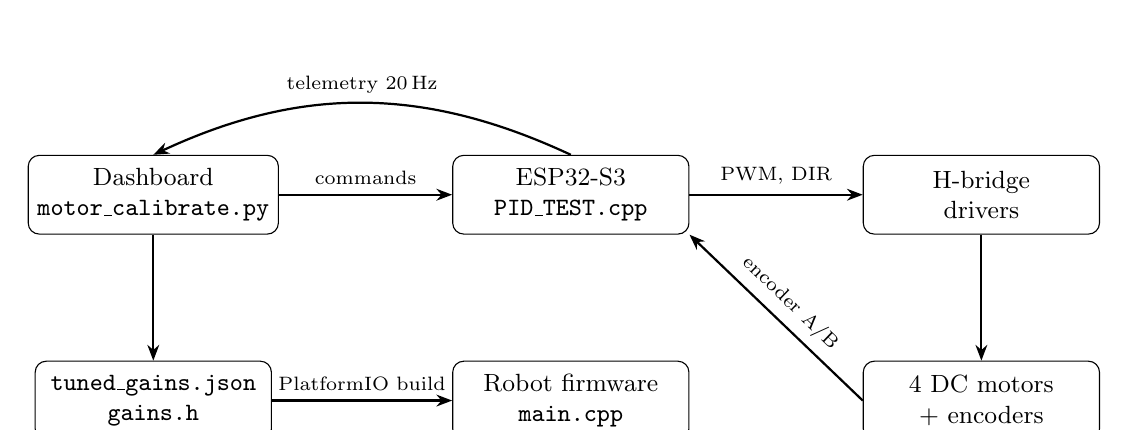
\begin{tikzpicture}[
  node distance=1.6cm and 2.2cm,
  box/.style={rectangle,draw,rounded corners,minimum width=3.0cm,minimum height=1.0cm,align=center,font=\small},
  arr/.style={-{Stealth[length=2mm]},thick}]
  \node[box] (gui) {Dashboard\\\code{motor\_calibrate.py}};
  \node[box,right=of gui] (esp) {ESP32-S3\\\code{PID\_TEST.cpp}};
  \node[box,right=of esp] (drv) {H-bridge\\drivers};
  \node[box,below=of drv] (mot) {4 DC motors\\+ encoders};
  \node[box,below=of gui] (file) {\code{tuned\_gains.json}\\\code{gains.h}};
  \node[box,below=of esp] (rob) {Robot firmware\\\code{main.cpp}};
  \draw[arr] (gui) -- node[above,font=\scriptsize]{commands} (esp);
  \draw[arr] (esp.north) to[bend right=25] node[above,font=\scriptsize]{telemetry 20\,Hz} (gui.north);
  \draw[arr] (esp) -- node[above,font=\scriptsize]{PWM, DIR} (drv);
  \draw[arr] (drv) -- (mot);
  \draw[arr] (mot.west) -- node[above,sloped,font=\scriptsize]{encoder A/B} (esp.south east);
  \draw[arr] (gui) -- (file);
  \draw[arr] (file) -- node[above,font=\scriptsize]{PlatformIO build} (rob);
\end{tikzpicture}
\caption{Tuning set-up. The dashboard commands the test firmware over USB serial and reads back the four wheel speeds; the result is written to files that the production firmware includes at build time.}\label{fig:arch}
\end{figure}

% ============================================================================
\chapter{Control Theory}
% ============================================================================

\section{Plant model: first order plus dead time with dead-band}
A permanent-magnet DC motor driven through a gearbox, with its inertial load, behaves for small variations around an operating point like a first-order lag. Static friction and the minimum voltage needed to overcome it add a dead-band, and sampling, driver and mechanical backlash add a short delay. The model used by the autotune is therefore
\begin{equation}
  G(s) = \frac{K\,e^{-\theta s}}{\tau s + 1}, \qquad \omega_{ss} = K\,(u - u_0)\ \ \text{for } u > u_0,\ \ \omega_{ss}=0 \text{ otherwise}. \label{eq:fopdt}
\end{equation}
For an open-loop PWM step of height $u$ applied at $t=0$ to a wheel at rest, the response is
\begin{equation}
  \omega(t) = K\,(u-u_0)\left(1 - e^{-(t-\theta)/\tau}\right),\qquad t\ge\theta, \label{eq:step}
\end{equation}
and zero before $\theta$. Three parameters, $K$, $\tau$ and $\theta$, plus the dead-band $u_0$, completely describe one motor in one direction. The model is linear only above the dead-band, which is why the identification uses several PWM levels and a straight-line fit of steady-state speed against PWM; the intercept of that line on the PWM axis is $u_0$.

\begin{figure}[H]
\centering
\begin{tikzpicture}[scale=1.0]
  \draw[->] (0,0) -- (7.2,0) node[right]{$t$};
  \draw[->] (0,0) -- (0,3.6) node[above]{$\omega$};
  \draw[dashed] (0,3) -- (7,3) node[right]{\small $\omega_{ss}=K(u-u_0)$};
  \draw[thick,blue] (0,0) -- (0.8,0) .. controls (1.8,2.4) and (3,2.9) .. (6.8,3);
  \draw[dotted] (0.8,0) -- (0.8,-0.3) node[below]{\small $\theta$};
  \draw[dotted] (2.0,0) -- (2.0,1.9);
  \draw[dotted] (0,1.9) -- (2.0,1.9);
  \node[below] at (2.0,-0.05) {\small $\theta+\tau$};
  \node[left] at (0,1.9) {\small $0.63\,\omega_{ss}$};
\end{tikzpicture}
\caption{Open-loop step response of the model~\eqref{eq:step}. $\theta$ is the delay before the speed starts to rise; after $\theta+\tau$ the speed has reached 63\,\% of its final value.}\label{fig:fopdt}
\end{figure}

\section{Identification from open-loop steps}
For each wheel and each direction the autotune applies a PWM step from rest, records the speed at $T_s$, fits a straight line to the steady-state speeds (Section~\ref{sec:ident-ols}) and fits $\tau$ and $\theta$ to each recorded trace (Section~\ref{sec:ident-fit}). This is done at several PWM levels. In the default configuration three levels are used first (150, 180, 210 counts), and then, when \code{ADAPTIVE\_LEVELS} is enabled, further levels are placed where the fitted model predicts the wheel will reach the speeds in \code{REFINE\_RPMS}:
\begin{equation}
  u_{\text{refine}} = \operatorname{round}\!\left(\min\{250,\ \max\{40,\ u_0 + v_{\text{target}}/K\}\}\right). \label{eq:refine}
\end{equation}
A refine level that falls within 8 counts of an existing level is skipped. The reason for the second stage is that the three initial levels all produce high speeds, so a model fitted only to them says little about the low-speed region where the dead-band and stiction dominate. After the refine steps the model is fitted again using all levels.

The program prints, per wheel and direction, the quantities \code{K}, \code{pwm0}, \code{tau}, \code{L}, the RMS fit error, a linearity error and the list of PWM levels used. \emph{Reading these lines is the main diagnostic of the whole process}: a large RMS fit error means the first-order model is a poor description (for example because of a slipping belt, a loose coupling or a battery that sags during the step); a large linearity error means the speed is not proportional to $(u-u_0)$ over the tested range.

\section{PI control law}
The controller used in both firmware images has the structure
\begin{equation}
  u[k] = \underbrace{F\,r[k] + \operatorname{sgn}(r[k])\,B}_{\text{feedforward}}
       + \underbrace{K_p\,e[k] + I[k]}_{\text{feedback}},\qquad e = r - \omega, \label{eq:pi}
\end{equation}
\begin{equation}
  I[k] = I[k-1] + K_i\,T_s\,e[k]. \label{eq:integ}
\end{equation}
The output is clamped to $[-255,255]$. A target of exactly zero forces $u=0$ and clears the integrator and the previous error, so a stopped wheel carries no wind-up into the next move. When the sign of the target changes, the integrator is also cleared, because an integrator filled for forward motion would act against the new direction.

\subsection{The feedforward term}
In steady state a wheel at speed $r$ needs $u = u_0 + r/K$. The feedforward term supplies exactly this when $F = 1/K$ and $B = u_0$. Two benefits follow. First, the integrator no longer has to build up the whole drive level, so the rise is faster and the overshoot smaller. Second, the dead-band is bridged immediately, which matters at low speed. A feedforward that is too large causes overshoot, because the loop then starts above the target; the autotune therefore starts from $F=0$ (offset only, \code{FF\_SCALE = 0}) and raises it afterwards only as far as the verification limits allow (Section~\ref{sec:verify-phase}).

\subsection{Separate forward and reverse gain sets}
A brushed motor with a gearbox rarely behaves identically in the two directions: brush position, gear mesh and the driver's inverted PWM in reverse all differ. The firmware therefore holds two complete sets $\{K_p,K_i,K_d,F,B\}$ per wheel. The set is chosen by the \emph{sign of the target}, not of the measured speed. In the serial protocol the forward set uses upper-case letters (\code{P I D F B}) and the reverse set the corresponding lower-case letters (\code{p i d f b}).

\subsection{Integrator limit and anti-windup}
In \code{PID\_TEST.cpp} the integrator state (in rpm$\cdot$s) is clamped to $\pm 255/K_i$, so that the integral contribution $K_i I$ can never exceed the full PWM range. (A comment in the source records that a fixed limit of 150 had allowed 750 PWM at $K_i=5$.) With $K_i = 0$ the integrator is held at zero. The production firmware uses a different but compatible scheme, stopping integration while the output is saturated and the error pushes further into saturation (conditional integration). Both prevent the long recovery tail that a wound-up integrator causes.

\subsection{Derivative action}
The test firmware supports $K_d$, but the autotune always sets it to zero, and the dashboard slider is limited to $0$--$2$. The reason is the quantisation in Equation~\eqref{eq:quant}: a single count of noise in one sample produces a change in the computed derivative of $\Delta\omega_{\min}/T_s \approx 32\rpm/\mathrm{s}$, multiplied by $K_d$. On a wheel whose steady-state ripple is already one count, derivative action turns that ripple into audible motor chatter. Derivative action is only worth trying with a filtered speed estimate, which this firmware does not have.

\section{PI tuning: the SIMC rules}
The gains are computed by the Skogestad IMC (SIMC) rules for a first-order-plus-dead-time process under PI control. For the plant~\eqref{eq:fopdt} with desired closed-loop time constant $\tau_c$:
\begin{equation}
  K_p = \frac{1}{K}\cdot\frac{\tau}{\tau_c+\theta},\qquad
  \tau_I = \min\{\tau,\ 4(\tau_c+\theta)\},\qquad
  K_i = \frac{K_p}{\tau_I}. \label{eq:simc}
\end{equation}
Equation~\eqref{eq:simc} is the standard published form and is what \code{simc\_pi} computes (Section~\ref{sec:simcpi}), followed by caps of 20 on $K_p$ and 60 on $K_i$. Because $K$ has units of rpm/PWM, $K_p$ has units of PWM/rpm, matching the firmware. The closed-loop response to a setpoint step is approximately a first-order lag with time constant $\tau_c$ plus the delay $\theta$. The single design parameter $\tau_c$ trades speed against robustness: decreasing it gives a faster response but a smaller gain and phase margin; the rule of thumb is $\tau_c \ge \theta$ (the ``tight control'' limit).

\subsection{Choice of $\tau_c$ and the shared value}
The dashboard sets $\tau_c$ once, as the largest of the lower bounds over every wheel and direction $m$ (\code{common\_tau\_c}, Section~\ref{sec:commontc}):
\begin{equation}
  \tau_c = \max_{m}\ \max\{\ \texttt{TAU\_C\_FACTOR}\cdot\tau_m,\ \ \texttt{TAU\_C\_L\_MULT}\cdot\theta_m\ \},\qquad \texttt{TAU\_C\_FACTOR}=0.25,\ \ \texttt{TAU\_C\_L\_MULT}=1.25. \label{eq:tauc}
\end{equation}
The value is common to all motors and both directions, so the slowest or most delayed plant sets it. The point of a common value is that the four wheels then respond with the same closed-loop speed, even if their plants differ. Different closed-loop speeds across the wheels would produce a transient yaw error whenever the robot accelerates, even if every wheel reached the same final speed.

\section{Closed-loop verification and detuning}
Model-based gains are only as good as the model, so each tuned pair is tested with a closed-loop step. The dashboard measures:
\begin{description}[noitemsep]
  \item[Overshoot] the maximum of the 3-point-smoothed speed above the target, as a percentage of the target;
  \item[Rise time (90\,\%)] the first time the smoothed speed reaches 90\,\% of the target (linearly interpolated between samples);
  \item[Settling time] the end of the last sample of the smoothed speed that lies outside a band of $\max\{5\,\%\ \text{of the target},\ 1.3\rpm\}$ around the target (0 if it never leaves the band);
  \item[Ripple] the peak-to-peak variation of the raw (unsmoothed) speed over the last 30\,\% of the window;
  \item[Final value] the mean raw speed over the same last 30\,\%.
\end{description}
A step passes when overshoot is at most \code{MAX\_OVERSHOOT\_PCT} (5\,\%) and ripple is at most \code{RIPPLE\_MAX\_RPM} (3\,rpm). If it fails, $K_p$ and $K_i$ are both multiplied by \code{DETUNE\_FACTOR} (0.75), the step is repeated, and this can occur at most \code{MAX\_DETUNE\_ROUNDS} (3) times. Scaling both gains by the same factor leaves the integral time $\tau_I=K_p/K_i$ unchanged and lowers only the loop bandwidth, which is the correct direction for reducing overshoot.

The verification target is \code{VERIFY\_RPM = 30}, reduced to 80\,\% of the largest steady-state speed reached in the identification if the wheel cannot reach 30\,rpm, with a floor of 10\,rpm.

\section{Feedforward speed-up}\label{sec:verify-phase}
After the PI settings pass (and only if the rise time was measurable and the overshoot within the limit), the autotune tries larger feedforward gains. It sets $F = f/K$ in turn for $f \in \{0.4,\,0.7,\,1.0\}$ (\code{FF\_SPEEDUP}) and repeats the verification step each time. A setting is kept only if it still passes the limits \emph{and} shortens the 90\,\% rise time by more than 20\,ms; the first setting that fails to improve ends the search, and the best setting so far is retained. The result is the fastest feedforward that does not cost overshoot or ripple.

\section{Speed sweep}\label{sec:sweep}
A linear model identified near the middle of the speed range does not guarantee uniform behaviour at the ends. The speed sweep commands all four motors together to each speed in \code{SWEEP\_SPEEDS} ($10, 20, 30, 50, 70, 100, 120\rpm$), forward and then reverse, with the \emph{current} gains. For each speed it reports the final speed of each wheel, the spread between the wheels and the largest miss from the target, and flags the speed if either exceeds \code{SWEEP\_SPREAD\_RPM} (2.5\,rpm; this is less than two encoder counts, see Equation~\eqref{eq:quant}). A flagged speed at the high end usually means the PWM has saturated: the largest speed a wheel can reach is approximately
\begin{equation}
  \omega_{\max} \approx K\,(u_{\max} - u_0),\qquad u_{\max} = 250\ \text{(production firmware)}\ \text{or}\ 255\ \text{(test firmware)}. \label{eq:wmax}
\end{equation}
Compare this with the identified $K$ and \code{pwm0} before concluding that a flag at 100 or 120\,rpm is a tuning problem.

% ============================================================================
\chapter[Test Firmware]{Test Firmware: \texttt{PID\_TEST.cpp}}
% ============================================================================

\section{Purpose}
\code{PID\_TEST.cpp} is a minimal firmware whose only job is to run four speed loops with runtime-adjustable gains and report the measured speeds. It deliberately contains none of the ROS code. It is flashed using the \code{pid\_test} PlatformIO environment (the name is configurable, see Table~\ref{tab:env}), and the dashboard talks to it at 115200\,baud.

\section{Control loop timing}
\code{loop()} polls the serial port on every pass and runs the control step only when at least \code{SAMPLE\_TIME\_MS = 50} milliseconds have elapsed since the last step. The elapsed time is measured and used as $dt$ in the speed computation and in the PI update, so a late iteration does not corrupt the speed estimate. The value 50\,ms \emph{must equal} \code{SAMPLE\_DT} in the Python file and \code{SPEED\_LOOP\_MS} in the production firmware, because the gains are tuned for that sampling period and because the identification fits are done on data at that spacing.

\subsection*{Blocking calls}
\begin{itemize}[noitemsep]
  \item \code{Serial.setTimeout(20)} in \code{setup()} bounds \code{readStringUntil('\textbackslash n')} to 20\,ms. The Arduino default is 1000\,ms, which would stall all four loops if a partial line arrived.
  \item The telemetry line is printed with \code{Serial.print} at 115200\,baud. At about 60--70 characters per line and 20 lines per second, the output uses about 14\,kbit/s of the 115.2\,kbit/s link, so the transmit buffer does not block.
  \item There are no interrupt service routines in this firmware. The encoder counting is done by the ESP32 pulse-counter hardware through the \code{ESP32Encoder} library, so no ISR safety concerns arise in user code.
\end{itemize}

\subsection*{Memory}
All state is statically allocated (four \code{SimplePID} objects, four encoder objects and small arrays). The only dynamic allocation is the Arduino \code{String} used for each received command line; command lines are short (under 20 characters), so heap fragmentation is not a practical concern, though a fixed \code{char} buffer would remove the issue entirely.

\section{The \texttt{SimplePID} class}
Listing~\ref{lst:pid} reproduces the control routine. The behaviour is as described in Chapter~3; the specific points of the implementation are:
\begin{enumerate}[noitemsep]
  \item \textbf{Open-loop mode} (\code{open\_loop = true}) bypasses the controller and returns \code{open\_pwm}. Integrator and previous error are cleared on every call so that the transition back to closed loop starts clean. This is the mode used for the autotune steps.
  \item \textbf{Zero target} returns 0 and clears state.
  \item \textbf{Gain-set selection} by the sign of the target, with a state reset on a direction change.
  \item \textbf{Integrator clamp} of $\pm255/K_i$.
  \item \textbf{Derivative} computed on the error with a one-sample difference. Because the target changes in steps, the first sample after a step produces a large derivative kick when $K_d \neq 0$ (another reason the autotune leaves it at 0).
  \item \textbf{Output} equals feedforward + P + I + D, clamped to $\pm255$ and truncated to an integer.
\end{enumerate}

\begin{lstlisting}[language=C++,caption={Core of \texttt{SimplePID::compute()} (abridged).},label={lst:pid}]
float error = tgt - current;
integral += error * dt;
if (KI > 0.0f) {
  float lim = 255.0f / KI;
  integral = constrain(integral, -lim, lim);
} else {
  integral = 0.0f;
}
float derivative = (dt > 0.0f) ? (error - prev_error) / dt : 0.0f;
prev_error = error;

float ff = tgt * FFG + (tgt > 0.0f ? FFO : -FFO);
float output = ff + (KP * error) + (KI * integral) + (KD * derivative);
return (int)constrain(output, -255.0f, 255.0f);
\end{lstlisting}

\section{Serial command protocol}
Commands are single text lines of the form
\begin{center}
\code{<cmd><sel><value>\textbackslash n}
\end{center}
where \code{cmd} is one character, \code{sel} is the selector (\code{A}, \code{1}, \code{2}, \code{3} or \code{4}) and \code{value} is a decimal number parsed with \code{toFloat()}. Lines of two characters or fewer are ignored. Table~\ref{tab:cmds} lists every command.

\begin{table}[H]
\centering
\caption{Serial commands accepted by \code{PID\_TEST.cpp}. Example: \code{TA30} sets all wheels to 30\,rpm; \code{P25.5} sets $K_p$ of wheel 2 (FR) to 5.5 --- note that the value starts right after the selector.}\label{tab:cmds}
\begin{tabular}{@{}clp{7.2cm}@{}}
\toprule
Command & Set & Effect\\
\midrule
\code{T} & target & Speed target in rpm, clamped to $\pm120$; selects closed loop (clears open-loop mode)\\
\code{P}, \code{I}, \code{D} & forward & $K_p$, $K_i$, $K_d$ used when the target is positive\\
\code{F} & forward & Feedforward gain, PWM per rpm\\
\code{B} & forward & Feedforward offset, PWM counts\\
\code{p}, \code{i}, \code{d} & reverse & $K_p$, $K_i$, $K_d$ used when the target is negative\\
\code{f}, \code{b} & reverse & Feedforward gain and offset for reverse\\
\code{M} & open loop & Raw PWM, clamped to $\pm255$, bypassing the controller; negative means reverse. Any later \code{T} returns to closed loop\\
\bottomrule
\end{tabular}
\end{table}

\warnbox{The command letters are case sensitive. In particular \code{P} sets the \emph{forward} proportional gain and \code{p} the \emph{reverse} one. The selector uses the digit characters \code{1}--\code{4}, not indices 0--3.}

\section{Telemetry}
Each control period the firmware prints one line:
\begin{center}
\code{Target:<rpm> FL:<rpm> FR:<rpm> RL:<rpm> RR:<rpm>}
\end{center}
The dashboard accepts a line only if it splits on whitespace into exactly five fields and the first contains \code{Target}; any other line (for example the banner printed at start-up) is ignored. \code{Target} is the \emph{most recently commanded} target, a single number for display, and not a per-wheel value. Speeds are in rpm after multiplication by the motor direction constant.

\section{Initial values}
All four controllers start with $K_p = 2.0$, $K_i = 5.0$, $K_d = 0$, $F = 3.4$ PWM/rpm, $B = 0$, for both directions. These are the dashboard's ``default'' values (\code{DEFAULT\_GAINS}) and are what \emph{RESET TO DEFAULT} restores.

% ============================================================================
\chapter[Host Software]{Host Software: \texttt{motor\_calibrate.py}}
% ============================================================================

\section{Dependencies and configuration}
The dashboard uses \code{pyserial}, \code{matplotlib}, \code{tkinter}, \code{python-dotenv} and the local module \code{autotune\_math}. All configuration comes from environment variables, optionally set in a \code{.env} file next to the script. Table~\ref{tab:env} lists them.

\begin{table}[H]
\centering
\caption{Environment variables read by the dashboard.}\label{tab:env}
\small
\begin{tabular}{@{}llp{6.2cm}@{}}
\toprule
Variable & Default & Meaning\\
\midrule
\code{SERIAL\_PORT} & \code{/dev/ttyUSB0} & Serial port of the ESP32 running \code{PID\_TEST}\\
\code{BAUD\_RATE} & 115200 & Must match \code{Serial.begin} in the test firmware\\
\code{GAINS\_FILE} & \code{tuned\_gains.json} & Where gains are saved and loaded\\
\code{ROBOT\_PROJECT} & (empty) & PlatformIO project folder of the robot firmware; needed for header generation and upload\\
\code{PIO\_CMD} & auto-detected & Path of the \code{pio} executable\\
\code{UPLOAD\_PORT} & (empty) & Port used for uploading; empty means \code{SERIAL\_PORT}\\
\code{PIO\_ENV\_ROBOT} & \code{robot} & \code{platformio.ini} environment for the robot firmware\\
\code{PIO\_ENV\_TEST} & \code{pid\_test} & \code{platformio.ini} environment for the test firmware\\
\code{GAINS\_HEADER} & \code{<ROBOT\_PROJECT>/include/gains.h}, or \code{gains.h} if \code{ROBOT\_PROJECT} is empty & C++ header written when gains are saved; empty string disables it\\
\code{AUTOLOAD\_GAINS} & 1 & If 1, load \code{GAINS\_FILE} at start-up; if 0, start from defaults\\
\bottomrule
\end{tabular}
\end{table}

\section{Tunable constants in the source}
Table~\ref{tab:const} lists the constants at the top of the file that shape the autotune. They are plain Python constants; change them in the source and restart.

\begin{table}[H]
\centering
\caption{Autotune constants in \code{motor\_calibrate.py}.}\label{tab:const}
\small
\begin{tabular}{@{}llp{6.4cm}@{}}
\toprule
Constant & Default & Role\\
\midrule
\code{SAMPLE\_DT} & 0.05\,s & Sample period; must equal \code{SAMPLE\_TIME\_MS} in firmware\\
\code{TEST\_PWMS} & 150, 180, 210 & Initial open-loop levels; all must clearly move the motor\\
\code{TEST\_DURATION} & 2.5\,s & Length of each step; should span several time constants\\
\code{SETTLE\_STOP} & 1.5\,s & Coast time between steps\\
\code{TAU\_C\_FACTOR} & 0.25 & $\tau_c \ge$ this $\times\ \tau$\\
\code{TAU\_C\_L\_MULT} & 1.25 & $\tau_c \ge$ this $\times\ \theta$ (1.0 is the SIMC limit)\\
\code{FF\_SCALE} & 0.0 & Starting feedforward, as a fraction of $1/K$\\
\code{FF\_SPEEDUP} & 0.4, 0.7, 1.0 & Feedforward fractions tried after PI passes\\
\code{ADAPTIVE\_LEVELS} & True & Add low-speed identification steps\\
\code{REFINE\_RPMS} & 15, 35 & Speeds the extra steps aim for\\
\code{MIN\_TEST\_PWM} & 40 & Never test below this PWM\\
\code{SWEEP\_SPEEDS} & 10 ... 120\,rpm & Speeds of the sweep\\
\code{SWEEP\_SPREAD\_RPM} & 2.5\,rpm & Tolerance for the sweep\\
\code{SWEEP\_AFTER\_AUTOTUNE} & True & Run the sweep automatically\\
\code{VERIFY\_RPM} & 30\,rpm & Verification step (capped at 80\,\% of fast open-loop speed)\\
\code{RIPPLE\_MAX\_RPM} & 3.0\,rpm & Peak-to-peak limit\\
\code{MAX\_OVERSHOOT\_PCT} & 5\,\% & Overshoot limit\\
\code{DETUNE\_FACTOR} & 0.75 & Multiplier on $K_p$, $K_i$ per detune round\\
\code{MAX\_DETUNE\_ROUNDS} & 3 & Maximum detune rounds\\
\code{AUTOTUNE\_REVERSE} & True & Also tune the reverse direction\\
\bottomrule
\end{tabular}
\end{table}

\section{Program structure}
The program has four cooperating parts:
\begin{enumerate}[noitemsep]
  \item \textbf{Main (GUI) thread.} Tk event loop and Matplotlib canvas. A timer calls \code{update\_plot()} every 100\,ms to redraw and to refresh the status line.
  \item \textbf{Serial reader thread} (\code{read\_serial}). Reads lines, parses the five fields, appends them to five 100-sample ring buffers (\code{collections.deque}) for the plot, and, when a capture is active, also appends the sample dictionary to the \code{capture} list.
  \item \textbf{Worker threads.} Autotune, step test, speed sweep, flashing and reconnect each run in their own daemon thread so the GUI stays responsive.
  \item \textbf{Shared state.} A set of module-level globals: \code{autotuning}, \code{abort\_autotune}, \code{refresh\_needed}, \code{status\_text}, \code{capture}, \code{flashing}, \code{updating\_gui}, and the per-motor dictionary \code{motor\_params}.
\end{enumerate}

\subsection{Per-motor memory}
\code{motor\_params} stores, for every wheel (keys \code{"1"}--\code{"4"}), the ten gains \code{P,I,D,F,B} and \code{Pr,Ir,Dr,Fr,Br} plus the last target \code{T}. The entry \code{"A"} stores only a target, so the \emph{All} selection can broadcast a speed but can never overwrite individual tuned gains.

\subsection{Preventing feedback loops in the GUI}
Moving a slider by software triggers its callback, which would send a command to the robot. The flag \code{updating\_gui} suppresses sending while the program is only moving sliders to show stored values; \code{sync\_sliders()} flushes pending Tk idle callbacks while the flag is still set so that no stray command is sent afterwards. While any worker is running, \code{autotuning} is True and \code{send\_command} refuses to send anything, so manual slider input cannot interfere with a test.

\subsection{Capture mechanism}
A step test records data by assigning a list to the global \code{capture}, sending the command, sleeping for \code{TEST\_DURATION}, and then swapping \code{capture} back to \code{None} and taking the recorded list. A test is rejected if it collected fewer than 80\,\% of the expected $T_{\text{duration}}/T_s$ samples: this protects the fit from serial dropouts and from a mismatch between \code{SAMPLE\_DT} and the firmware.

\section{Graphical interface}
Figure~\ref{fig:gui} shows the layout (to be replaced by a screenshot). The left column holds the controls, the right the live plot of target and four wheel speeds (fixed vertical range $\pm150$\,rpm).

\plotph{Screenshot of the dashboard during a step test.}{fig:gui}

Table~\ref{tab:buttons} explains every control.

\begin{table}[H]
\centering
\caption{Dashboard controls.}\label{tab:buttons}
\small
\begin{tabular}{@{}lp{9.5cm}@{}}
\toprule
Control & Function\\
\midrule
Motor radio buttons & Choose ALL (target only), FL, FR, RL or RR; the sliders then show and edit that wheel\\
Forward / Reverse gains & Choose which gain set the $K_p$, $K_i$, $K_d$ sliders edit\\
Target RPM slider and box & Send a closed-loop target ($\pm120$\,rpm); the box accepts a value and Enter\\
$K_p$, $K_i$, $K_d$ sliders & Edit the selected wheel and direction; disabled when ALL is selected\\
PAUSE PLOT & Freezes the plot (data keep flowing)\\
STOP MOTORS & Aborts any test, zeroes all targets, sends \code{TA0}\\
AUTOTUNE & Full procedure for the selected wheel or for all\\
SAVE GAINS & Writes JSON and the C++ header\\
IMPORT GAINS & Loads a JSON file and applies it\\
RESET TO DEFAULT & Restores \code{DEFAULT\_GAINS} on all wheels (file on disk untouched)\\
STEP TEST & Closed-loop $\pm30$\,rpm steps on all wheels with the current gains; prints metrics\\
SPEED SWEEP & The seven-speed sweep, forward and reverse\\
UPLOAD PID TEST & Builds and flashes the test firmware, then reconnects\\
SAVE + UPLOAD ROBOT FIRMWARE & Saves gains, then builds and flashes the robot firmware\\
RECONNECT & Reopens the serial port after the firmware was changed elsewhere\\
\bottomrule
\end{tabular}
\end{table}

% ============================================================================
\chapter[Numerical Routines]{Numerical Routines: \texttt{autotune\_math.py}}\label{ch:math}
% ============================================================================

\section{Role of the module}
\code{autotune\_math.py} is a pure-Python module. It imports only the standard \code{math} library and touches no hardware, so each routine can be run and tested offline (Section~\ref{sec:mathsim} does exactly that). The dashboard calls the four public functions of Table~\ref{tab:mathfun}. The module docstring fixes the plant model of Equation~\eqref{eq:fopdt}, $\omega = K(u-u_0)$ with a first-order lag $\tau$ and a dead time $L$, and the firmware feedforward rule $u = rF + \operatorname{sgn}(r)\,u_0$ with $F=\texttt{FF\_SCALE}/K$.

\begin{table}[H]
\centering
\caption{Public functions of \code{autotune\_math.py}.}\label{tab:mathfun}
\small
\begin{tabular}{@{}p{4.6cm}p{4.2cm}p{5.2cm}@{}}
\toprule
Function & Called from & Purpose\\
\midrule
\code{identify(levels, rpms, dt)} & \code{identify\_motor} & Dead-band line ($K$, $u_0$), then $\tau$ and $L$ (Sections~\ref{sec:ident-ols}, \ref{sec:ident-fit})\\
\code{common\_tau\_c(plants, f, m)} & \code{autotune\_worker} & One shared $\tau_c$ (Section~\ref{sec:commontc})\\
\code{simc\_pi(K, tau, L, tau\_c=)} & \code{autotune\_worker} & $K_p$, $K_i$ (Section~\ref{sec:simcpi})\\
\code{step\_metrics(rpm, target, dt)} & \code{\_verify\_step}, \code{step\_test\_worker}, \code{speed\_sweep} & Overshoot, rise, settling, ripple, final value (Section~\ref{sec:stepmetrics})\\
\bottomrule
\end{tabular}
\end{table}

\section{Helper functions}
\subsection*{Smoothing}
\code{\_smooth(x, n=3)} is a centred moving average whose window shrinks at both ends:
\begin{equation}
  \tilde y_i=\frac{1}{|W_i|}\sum_{j\in W_i}y_j,\qquad W_i=\{\max(0,i-1),\dots,\min(N-1,i+1)\}.
\end{equation}
It introduces no net delay but spreads a step edge over three samples (150\,ms) and divides an isolated one-sample glitch by three: a one-count error of 1.6\,rpm becomes 0.53\,rpm. It is non-causal and is used only on recorded data.

\subsection*{Steady value}
\code{\_steady(x, frac=0.3)} is the mean of the last $M=\max\{3,\lfloor0.3N\rfloor\}$ samples. For a 2.5\,s record ($N=50$) that is the last 15 samples (0.75\,s). It assumes the response has settled by then; see Section~\ref{sec:mathreview}.

\subsection*{Level crossing}
\code{\_crossing(x, level, dt)} returns the first time the series reaches \code{level}, linearly interpolated. Sample $i$ is placed at $t_i=(i+1)\,dt$ and the series is taken to start at $(0,0)$:
\begin{equation}
  t^\ast=t_{i-1}+\frac{\ell-y_{i-1}}{y_i-y_{i-1}}\,(t_i-t_{i-1}).
\end{equation}
If the level is never reached it raises \code{ValueError}, which \code{step\_metrics} turns into ``rise = never''.

\section{Gain and dead-band by regression}\label{sec:ident-ols}
\code{identify} first takes the steady value $s_k$ of every open-loop step $k$ and keeps the points $(p_k,s_k)$ with $s_k\ge 3$\,rpm, where $p_k$ is the PWM level. Fewer than two points raise ``motor barely moves: raise TEST\_PWMS''. An ordinary least-squares line through the kept points gives
\begin{equation}
  K=\frac{\sum_k (p_k-\bar p)(s_k-\bar s)}{\sum_k (p_k-\bar p)^2},\qquad
  u_0=\bar p-\frac{\bar s}{K},\qquad
  e_{\text{lin}}=\max_k\bigl|s_k-K(p_k-u_0)\bigr|.
\end{equation}
$u_0$ is the PWM-axis intercept of the line, an extrapolation to zero speed. If the true curve bends near the dead-band (stiction, driver non-linearity) the extrapolation is biased, which is why the refine stage adds levels that produce 15 and 35\,rpm. A non-positive $K$ raises ``check encoder polarity / PWM levels''. The regression is unweighted.

\section{Time constant and dead time by grid search}\label{sec:ident-fit}
For each step with a steady speed of at least 10\,rpm (or, if no step reaches 10\,rpm, for the fastest step), \code{\_fit\_fopdt} fits the model of Equation~\eqref{eq:step} with the steady value held fixed at the measured $\bar y$ and only $\tau$ and $L$ free:
\begin{equation}
  \hat y(t_j;\tau,L)=\begin{cases}0 & t_j\le L\\ \bar y\,\bigl[1-e^{-(t_j-L)/\tau}\bigr] & t_j>L\end{cases},\qquad
  (\hat\tau,\hat L)=\arg\min_{(\tau,L)\in\mathcal G}\ \sum_j\bigl(y_j-\hat y(t_j)\bigr)^2 .
\end{equation}
The search grid $\mathcal G$ is the product of 75 time constants $\tau_i=0.03\cdot1.06^{\,i}$ (0.03 to 2.24\,s, 6\,\% steps) and 33 delays $L_k=0.0125\,k$ (0 to 0.4\,s, a quarter of the sample period). That is 2475 candidate pairs, about 124\,000 exponentials per fit, a fraction of a second in plain Python. The function returns $\hat\tau$, $\max(\hat L,\,dt)$ and the rms residual $\sqrt{\mathrm{SSE}/N}$.

\code{identify} then takes the median of the per-step $\tau$ values and of the per-step $L$ values separately (element \code{len//2} of the sorted list, the upper median when the count is even) and reports the worst rms residual. Taking the median makes the result robust to one bad step.

\paragraph{What $L$ means.} The speed sample at $t_j$ is the encoder change over the preceding 50\,ms, i.e.\ the mean speed over that interval, which lags the true speed by about $dt/2=25$\,ms. The identified $L$ is therefore the motor's own delay plus about 25\,ms, and it cannot fall below $dt=50$\,ms because of the floor. In the simulated example of Section~\ref{sec:mathsim}, a true delay of 60\,ms was identified as 87.5\,ms.

\section{The shared closed-loop time constant}\label{sec:commontc}
\begin{equation}
  \tau_c=\max_{m}\ \max\bigl\{\ \max(l_{\text{mult}},1)\,L_m,\ \ f\,\tau_m\ \bigr\},
\end{equation}
over every wheel and direction $m$, with $f=\texttt{TAU\_C\_FACTOR}=0.25$ and $l_{\text{mult}}=\texttt{TAU\_C\_L\_MULT}=1.25$ in the dashboard. The most delayed or slowest plant therefore sets $\tau_c$ for all eight loops, so the four wheels respond alike. The module defaults ($f=0.5$, $l_{\text{mult}}=2.0$) are older, more cautious values that the dashboard overrides.

\section{SIMC gains}\label{sec:simcpi}
With a shared value, \code{simc\_pi} uses $\tau_c\leftarrow\max(\tau_c,L)$ and returns
\begin{equation}
  K_p=\min\Bigl\{\frac{\tau}{K(\tau_c+L)},\ 20\Bigr\},\qquad
  K_i=\min\Bigl\{\frac{\tau/\,[K(\tau_c+L)]}{\min\{\tau,\ 4(\tau_c+L)\}},\ 60\Bigr\},
\end{equation}
where the numerator of the second fraction is the uncapped proportional gain. The caps equal the ranges of the dashboard sliders (0 to 20 and 0 to 60). The product $K_pK=\tau/(\tau_c+L)$ is the same for all plants with the same $\tau$ and $L$, so a stronger motor simply gets a proportionally smaller $K_p$. If \code{tau\_c} is not passed, the function falls back to $\max(2L,\,f\tau)$; the dashboard always passes it.

\section{Step metrics}\label{sec:stepmetrics}
\code{step\_metrics(rpm, target, dt)} evaluates a closed-loop step from rest to a positive target. With $\tilde y$ the 3-point-smoothed series and $y$ the raw one:
\begin{center}
\small
\begin{tabular}{@{}lp{9.6cm}@{}}
\toprule
Output & Definition\\
\midrule
\code{overshoot\_pct} & $\max\{0,\ (\max\tilde y-r)/r\times100\}$\\
\code{rise90\_s} & first time $\tilde y$ reaches $0.9\,r$ (Section~\ref{sec:ident-ols}'s crossing rule), or \code{None}\\
\code{settle\_s} & $dt\times(1+\text{index of the last sample with } |\tilde y-r|>\text{band})$, or 0; band $=\max(0.05\,r,\ 1.3\rpm)$\\
\code{final\_rpm} & mean of the raw $y$ over the last $\max\{3,\lfloor0.3N\rfloor\}$ samples\\
\code{ripple\_pp} & $\max-\min$ of the raw $y$ over the same samples\\
\bottomrule
\end{tabular}
\end{center}
The reverse tests multiply the recorded speeds by $-1$ before calling the function, so the target is always positive.

\section{Worked example on a simulated motor}\label{sec:mathsim}
To show the routines working end to end, the unmodified \code{autotune\_math.py} was run on a \emph{simulated} motor. This is an illustration with an assumed plant, not a measurement of the robot. The plant has $K=0.60$\,rpm/PWM (so $K(250-45)\approx123$\,rpm at the top PWM, consistent with the 120\,rpm limit), $u_0=45$, $\tau=0.18$\,s and a 60\,ms delay. It is observed through a 748 count/rev encoder every 50\,ms, so the speed is quantised in steps of 1.60\,rpm. The simulation repeats the sequence of \code{identify\_motor} (levels 150, 180, 210, then refine levels for 15 and 35\,rpm) and of \code{verify\_motor} (PI rounds, then the feedforward speed-up). Replace these tables with your own console output (Table~\ref{tab:ident} onward).

\subsection{Identification}
\begin{table}[H]
\centering
\caption{True and identified parameters of the simulated motor.}
\small
\begin{tabular}{@{}lcc@{}}
\toprule
Quantity & True & Identified\\
\midrule
$K$ [rpm/PWM] & 0.600 & 0.601\\
$u_0$ [PWM] & 45.0 & 45.1\\
$\tau$ [s] & 0.180 & 0.172\\
$L$ [s] & 0.060 (+0.025 measurement lag) & 0.0875\\
Fit rms [rpm] & -- & 0.82\\
Linearity error [rpm] & -- & 0.037\\
PWM levels used & -- & 70, 103, 150, 180, 210\\
\bottomrule
\end{tabular}
\end{table}

\begin{figure}[H]
\centering
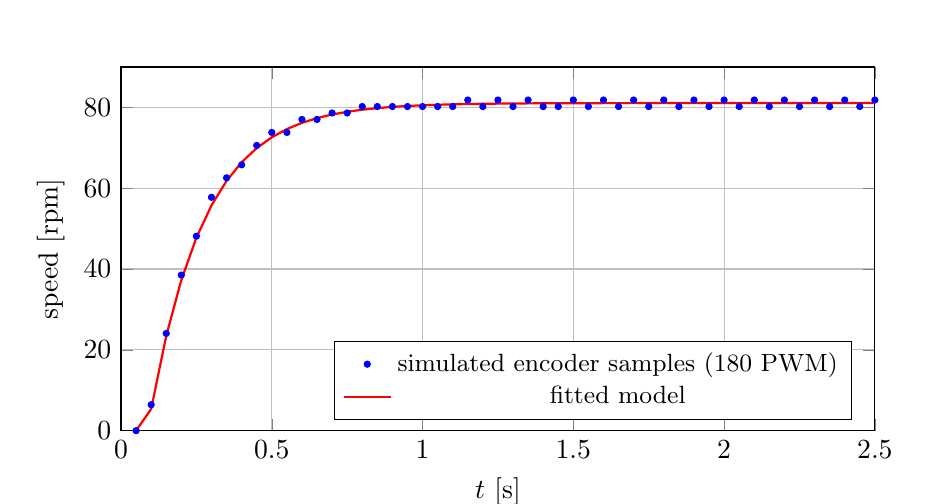
\begin{tikzpicture}
\begin{axis}[width=0.92\textwidth,height=6.2cm,xlabel={$t$ [s]},ylabel={speed [rpm]},grid=major,xmin=0,xmax=2.5,ymin=0,legend pos=south east,legend style={font=\small}]
\addplot[only marks,mark=*,mark size=1.1pt,blue] coordinates {(0.05,0.0) (0.1,6.42) (0.15,24.06) (0.2,38.5) (0.25,48.13) (0.3,57.75) (0.35,62.57) (0.4,65.78) (0.45,70.59) (0.5,73.8) (0.55,73.8) (0.6,77.01) (0.65,77.01) (0.7,78.61) (0.75,78.61) (0.8,80.21) (0.85,80.21) (0.9,80.21) (0.95,80.21) (1.0,80.21) (1.05,80.21) (1.1,80.21) (1.15,81.82) (1.2,80.21) (1.25,81.82) (1.3,80.21) (1.35,81.82) (1.4,80.21) (1.45,80.21) (1.5,81.82) (1.55,80.21) (1.6,81.82) (1.65,80.21) (1.7,81.82) (1.75,80.21) (1.8,81.82) (1.85,80.21) (1.9,81.82) (1.95,80.21) (2.0,81.82) (2.05,80.21) (2.1,81.82) (2.15,80.21) (2.2,81.82) (2.25,80.21) (2.3,81.82) (2.35,80.21) (2.4,81.82) (2.45,80.21) (2.5,81.82)};
\addplot[thick,red,mark=none] coordinates {(0.05,0.0) (0.1,5.36) (0.15,23.49) (0.2,37.28) (0.25,47.77) (0.3,55.74) (0.35,61.81) (0.4,66.42) (0.45,69.93) (0.5,72.6) (0.55,74.63) (0.6,76.17) (0.65,77.34) (0.7,78.24) (0.75,78.91) (0.8,79.43) (0.85,79.82) (0.9,80.12) (0.95,80.35) (1.0,80.52) (1.05,80.65) (1.1,80.75) (1.15,80.83) (1.2,80.89) (1.25,80.93) (1.3,80.96) (1.35,80.99) (1.4,81.01) (1.45,81.02) (1.5,81.03) (1.55,81.04) (1.6,81.05) (1.65,81.05) (1.7,81.06) (1.75,81.06) (1.8,81.06) (1.85,81.06) (1.9,81.07) (1.95,81.07) (2.0,81.07) (2.05,81.07) (2.1,81.07) (2.15,81.07) (2.2,81.07) (2.25,81.07) (2.3,81.07) (2.35,81.07) (2.4,81.07) (2.45,81.07) (2.5,81.07)};
\legend{simulated encoder samples (180 PWM),fitted model}
\end{axis}
\end{tikzpicture}
\caption{Open-loop step at 180 PWM on the simulated motor and the fitted model ($\hat\tau=0.183$\,s, $\hat L=0.0875$\,s). The steps in the data are single encoder counts (1.6\,rpm). Simulation, not measured data.}\label{fig:simfit}
\end{figure}

\subsection{Gains and verification}
The shared $\tau_c$ is $\max(1.25\times0.0875,\ 0.25\times0.172)=0.109$\,s. \code{simc\_pi} then gives $K_p=1.46$ and $K_i=8.46$, with feedforward offset $B=45.1$ and $F=0$ (\code{FF\_SCALE}\,$=0$).

\begin{table}[H]
\centering
\caption{\code{verify\_motor} on the simulated motor, 30\,rpm step. A round passes if overshoot $\le5$\,\% and ripple $\le3$\,rpm.}
\small
\begin{tabular}{@{}lccccccc@{}}
\toprule
Round & $K_p$ & $K_i$ & Overshoot [\%] & Rise 90\,\% [s] & Settle [s] & Ripple [rpm] & Result\\
\midrule
1 & 1.46 & 8.46 & 7.0 & 0.28 & 0.50 & 1.6 & fail, detune\\
2 & 1.09 & 6.35 & 1.6 & 0.39 & 0.45 & 1.6 & pass\\
FF 0.4/K & 1.09 & 6.35 & 12.3 & 0.27 & 0.70 & 1.6 & fail, stop\\
\bottomrule
\end{tabular}
\end{table}

The first round overshoots by 7\,\%, so both gains are multiplied by 0.75 and the second round passes. The feedforward search then tries $F=0.4/K=0.666$ and fails on overshoot (12.3\,\%), which ends the search, so the final feedforward stays at zero.

\begin{figure}[H]
\centering
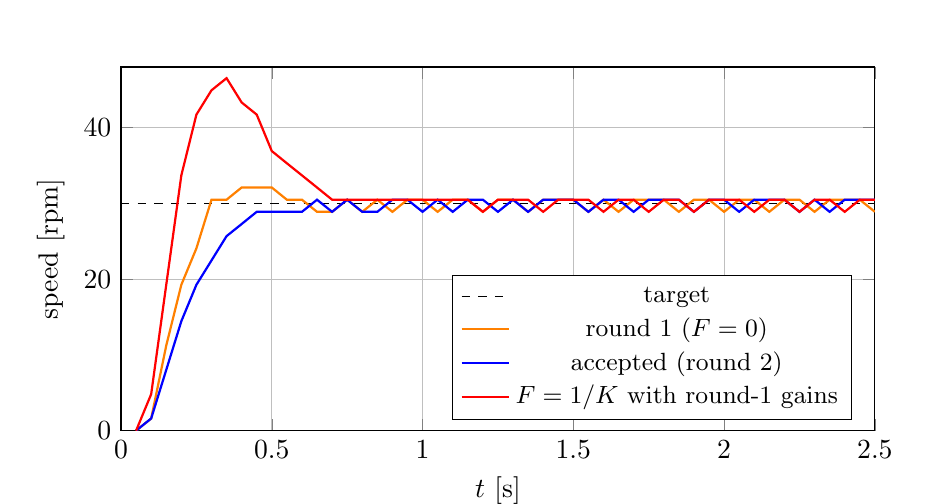
\begin{tikzpicture}
\begin{axis}[width=0.92\textwidth,height=6.2cm,xlabel={$t$ [s]},ylabel={speed [rpm]},grid=major,xmin=0,xmax=2.5,ymin=0,ymax=48,legend pos=south east,legend style={font=\small}]
\addplot[dashed,black,mark=none] coordinates {(0,30)(2.5,30)};
\addplot[thick,orange,mark=none] coordinates {(0.05,0.0) (0.1,1.6) (0.15,11.23) (0.2,19.25) (0.25,24.06) (0.3,30.48) (0.35,30.48) (0.4,32.09) (0.45,32.09) (0.5,32.09) (0.55,30.48) (0.6,30.48) (0.65,28.88) (0.7,28.88) (0.75,30.48) (0.8,28.88) (0.85,30.48) (0.9,28.88) (0.95,30.48) (1.0,30.48) (1.05,28.88) (1.1,30.48) (1.15,30.48) (1.2,28.88) (1.25,30.48) (1.3,30.48) (1.35,28.88) (1.4,30.48) (1.45,30.48) (1.5,30.48) (1.55,28.88) (1.6,30.48) (1.65,28.88) (1.7,30.48) (1.75,30.48) (1.8,30.48) (1.85,28.88) (1.9,30.48) (1.95,30.48) (2.0,28.88) (2.05,30.48) (2.1,30.48) (2.15,28.88) (2.2,30.48) (2.25,30.48) (2.3,28.88) (2.35,30.48) (2.4,30.48) (2.45,30.48) (2.5,28.88)};
\addplot[thick,blue,mark=none] coordinates {(0.05,0.0) (0.1,1.6) (0.15,8.02) (0.2,14.44) (0.25,19.25) (0.3,22.46) (0.35,25.67) (0.4,27.27) (0.45,28.88) (0.5,28.88) (0.55,28.88) (0.6,28.88) (0.65,30.48) (0.7,28.88) (0.75,30.48) (0.8,28.88) (0.85,28.88) (0.9,30.48) (0.95,30.48) (1.0,28.88) (1.05,30.48) (1.1,28.88) (1.15,30.48) (1.2,30.48) (1.25,28.88) (1.3,30.48) (1.35,28.88) (1.4,30.48) (1.45,30.48) (1.5,30.48) (1.55,28.88) (1.6,30.48) (1.65,30.48) (1.7,28.88) (1.75,30.48) (1.8,30.48) (1.85,30.48) (1.9,28.88) (1.95,30.48) (2.0,30.48) (2.05,28.88) (2.1,30.48) (2.15,30.48) (2.2,30.48) (2.25,28.88) (2.3,30.48) (2.35,28.88) (2.4,30.48) (2.45,30.48) (2.5,30.48)};
\addplot[thick,red,mark=none] coordinates {(0.05,0.0) (0.1,4.81) (0.15,19.25) (0.2,33.69) (0.25,41.71) (0.3,44.92) (0.35,46.52) (0.4,43.32) (0.45,41.71) (0.5,36.9) (0.55,35.29) (0.6,33.69) (0.65,32.09) (0.7,30.48) (0.75,30.48) (0.8,30.48) (0.85,30.48) (0.9,30.48) (0.95,30.48) (1.0,30.48) (1.05,30.48) (1.1,30.48) (1.15,30.48) (1.2,28.88) (1.25,30.48) (1.3,30.48) (1.35,30.48) (1.4,28.88) (1.45,30.48) (1.5,30.48) (1.55,30.48) (1.6,28.88) (1.65,30.48) (1.7,30.48) (1.75,28.88) (1.8,30.48) (1.85,30.48) (1.9,28.88) (1.95,30.48) (2.0,30.48) (2.05,30.48) (2.1,28.88) (2.15,30.48) (2.2,30.48) (2.25,28.88) (2.3,30.48) (2.35,30.48) (2.4,28.88) (2.45,30.48) (2.5,30.48)};
\legend{target,round 1 ($F=0$),accepted (round 2),$F=1/K$ with round-1 gains}
\end{axis}
\end{tikzpicture}
\caption{Closed-loop 30\,rpm step on the simulated motor. Round 1 overshoots, the detuned round 2 is accepted, and adding feedforward to a plain PI loop makes the overshoot worse. Simulation, not measured data.}\label{fig:simcl}
\end{figure}

\subsection{Effect of $\tau_c$ and of feedforward}
\begin{table}[H]
\centering
\caption{Effect of the design parameter $\tau_c$ (simulated motor, $F=0$, 30\,rpm step). Values of $\tau_c$ below $L$ give the same gains, because of the $\max(\tau_c,L)$ floor.}
\small
\begin{tabular}{@{}cccccc@{}}
\toprule
$\tau_c$ [s] & $K_p$ & $K_i$ & Overshoot [\%] & Rise 90\,\% [s] & Settle [s]\\
\midrule
0.06 & 1.64 & 9.51 & 10.5 & 0.25 & 0.50\\
0.08 & 1.64 & 9.51 & 10.5 & 0.25 & 0.50\\
0.12 & 1.38 & 8.02 & 3.4 & 0.30 & 0.30\\
0.18 & 1.07 & 6.22 & 1.6 & 0.41 & 0.45\\
0.30 & 0.74 & 4.30 & 1.6 & 0.76 & 0.85\\
0.50 & 0.49 & 2.83 & 0.0 & 1.22 & 1.60\\
\bottomrule
\end{tabular}
\end{table}

\begin{table}[H]
\centering
\caption{Effect of the feedforward fraction $f$ ($F=f/K$) with the round-1 gains and no detuning (simulated motor).}
\small
\begin{tabular}{@{}cccccc@{}}
\toprule
$f$ & $F$ [PWM/rpm] & Overshoot [\%] & Rise 90\,\% [s] & Settle [s] & Ripple [rpm]\\
\midrule
0.0 & 0.000 & 7.0 & 0.28 & 0.50 & 1.6\\
0.4 & 0.666 & 23.0 & 0.22 & 0.55 & 1.6\\
0.7 & 1.165 & 37.3 & 0.20 & 0.60 & 1.6\\
1.0 & 1.665 & 49.7 & 0.18 & 0.65 & 1.6\\
\bottomrule
\end{tabular}
\end{table}

Three things follow, and all are properties of this simulated plant. (i) Identification recovers $K$ and $u_0$ to better than 0.5\,\% and $\tau$ to about 5\,\%. (ii) With $l_{\text{mult}}=1.25$ the autotune starts at the edge of acceptable overshoot and typically needs one detune round, while $\tau_c$ of about 1.5 to 2 times $L$ would start closer to the final answer (the dashboard comment notes that 2.0 was the earlier setting). (iii) A plain PI loop with feedforward overshoots more as $f$ grows, because the integrator accumulates error during the rise even though feedforward already supplies the steady-state drive. The speed-up search therefore stops at its first step here. Feedforward only pays off with a setpoint ramp or filter, or with setpoint weighting on the proportional term; whether your motors behave the same way is visible in the console lines ``FF 0.4/K''.


% ============================================================================
\chapter{The Autotune Algorithm Step by Step}
% ============================================================================

\section{Overview}
The autotune is one function, \code{autotune\_worker(selection)}, running in a thread. Figure~\ref{fig:flow} summarises it.

\begin{figure}[H]
\centering
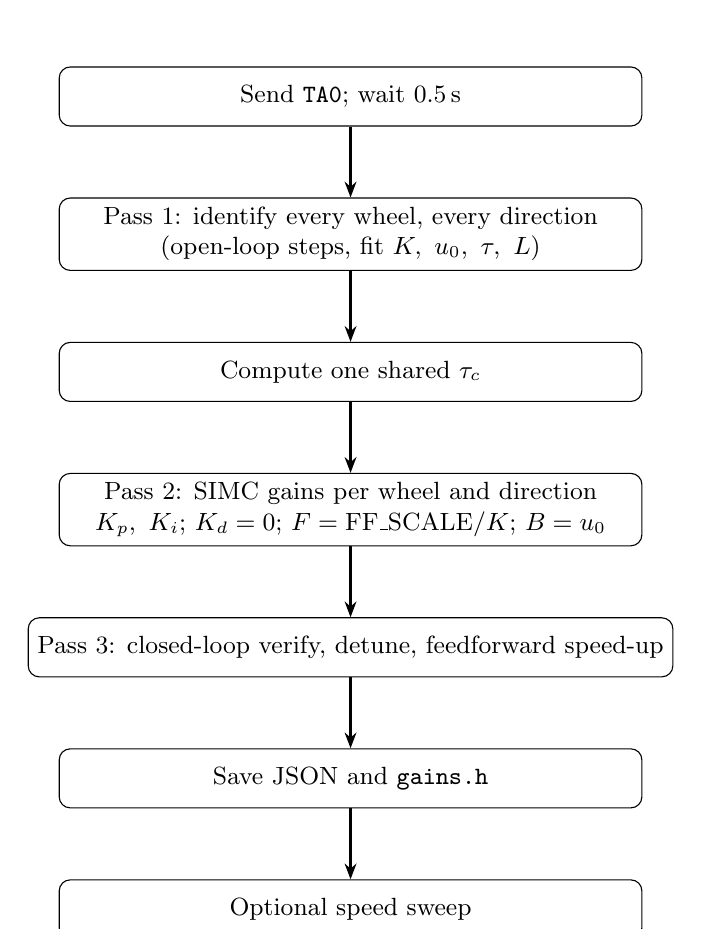
\begin{tikzpicture}[node distance=0.9cm,
  b/.style={rectangle,draw,rounded corners,minimum width=7.4cm,minimum height=0.75cm,align=center,font=\small},
  arr/.style={-{Stealth[length=2mm]},thick}]
  \node[b] (a) {Send \code{TA0}; wait 0.5\,s};
  \node[b,below=of a] (b1) {Pass 1: identify every wheel, every direction\\(open-loop steps, fit $K,\ u_0,\ \tau,\ L$)};
  \node[b,below=of b1] (c) {Compute one shared $\tau_c$};
  \node[b,below=of c] (d) {Pass 2: SIMC gains per wheel and direction\\$K_p,\ K_i$; $K_d=0$; $F=\mathrm{FF\_SCALE}/K$; $B=u_0$};
  \node[b,below=of d] (e) {Pass 3: closed-loop verify, detune, feedforward speed-up};
  \node[b,below=of e] (f) {Save JSON and \code{gains.h}};
  \node[b,below=of f] (g) {Optional speed sweep};
  \foreach \x/\y in {a/b1,b1/c,c/d,d/e,e/f,f/g} \draw[arr] (\x) -- (\y);
\end{tikzpicture}
\caption{Flow of \code{autotune\_worker}. Any step can be aborted with STOP MOTORS.}\label{fig:flow}
\end{figure}

\section{Pass 1: identification}
For each wheel and direction \code{identify\_motor(m, d)} performs:
\begin{enumerate}[noitemsep]
  \item \textbf{Stage 1.} For each PWM in \code{TEST\_PWMS}: send \code{M<m><pwm>} (reverse uses $-\mathrm{pwm}$), record 2.5\,s of speed, send \code{T<m>0}, then \code{wait\_stopped}, which sleeps 1.5\,s and waits a further 1.5\,s if the last measured speed is still above 2\,rpm.
  \item Fit the model to the three traces (reverse data are sign-flipped so the fit always works on positive magnitudes).
  \item \textbf{Stage 2} (if \code{ADAPTIVE\_LEVELS}): for each speed in \code{REFINE\_RPMS} compute the PWM from Equation~\eqref{eq:refine}, skip it if within 8 counts of an existing level, otherwise run the step. Refit with all levels.
  \item Print the result line.
\end{enumerate}
If at any point the user presses STOP MOTORS, the function returns \code{None} and the whole autotune reports ``aborted''.

The three initial levels are all high (150--210), which is a deliberate choice: the motors must clearly move so that the step shows a clean rise. The disadvantage is that 150--210 counts without load produce speeds well above the range the robot will be driven in, hence the refine stage.

\section{Pass 2: computing gains}
With all plants identified, a single $\tau_c$ is computed over all of them (Equation~\eqref{eq:tauc}) and printed. Then for each wheel and direction the SIMC gains are computed and stored:
\begin{center}
$K_p,\ K_i \leftarrow \texttt{simc\_pi}(K,\tau,\theta,\tau_c),\quad K_d \leftarrow 0,\quad F \leftarrow \texttt{FF\_SCALE}/K,\quad B \leftarrow u_0.$
\end{center}
$K_p$ and $K_i$ are rounded to two decimals, $F$ to three and $B$ to one. If \code{AUTOTUNE\_REVERSE} is off, the reverse set is copied from the forward set.

\section{Pass 3: verification}\label{sec:verify-pass}
For each (wheel, direction) the verification of Section~\ref{sec:verify-phase} is run as described in Chapter~3: PI detune loop first, then the feedforward speed-up. Each test pushes all ten gains to the wheel with \code{push\_gains} (10\,ms between lines to stay below the ESP32 receive buffer), runs the step, waits for the wheel to stop, computes the metrics and prints them. The final feedforward is pushed again at the end.

\section{Saving}
On success the dashboard calls \code{save\_gains()}, which (i) copies any existing JSON to \code{.bak}, (ii) writes the new JSON, and (iii) writes the header \code{gains.h}. The JSON structure is
\begin{lstlisting}[language=Python]
{ "1": {"P":..,"I":..,"D":..,"F":..,"B":..,"Pr":..,"Ir":..,"Dr":..,"Fr":..,"Br":..},
  "2": {...}, "3": {...}, "4": {...} }
\end{lstlisting}
and the header is
\begin{lstlisting}[language=C++]
struct Gain { float kp, ki, kd, ff, off; };
struct MotorGains { Gain fwd, rev; };
constexpr MotorGains GAINS_FL = {{kp, ki, kd, ff, off}, {kp, ki, kd, ff, off}};
// ... GAINS_FR, GAINS_RL, GAINS_RR
\end{lstlisting}
The production firmware includes this header and builds its per-wheel controllers from it. Importing an older JSON file that lacks the reverse set is supported: the reverse values are filled from the forward ones.

\section{Estimated duration}
A rough estimate from the constants (not measured): each open-loop step takes 2.5\,s plus 1.5--3\,s of settling, five steps per wheel and direction give about 20--25\,s, and the closed-loop verifications take 4--7 steps of similar length. With four wheels and both directions the identification takes roughly 3 minutes and the verification up to about 4 minutes, plus about 1 minute for the sweep. Allow 5--10 minutes in total. \todo{Replace with the measured duration.}

% ============================================================================
\chapter{Other Functions of the Dashboard}
% ============================================================================

\section{Step test}
\code{step\_test\_worker} applies a closed-loop step from 0 to $+30$ and then to $-30\rpm$ on \emph{all} wheels simultaneously with the \emph{current} gains and prints the five metrics per wheel and direction together with the gains in use. Its intended use is a before/after comparison: run it after RESET TO DEFAULT, then after IMPORT or AUTOTUNE, and compare overshoot, rise time and ripple.

\section{Speed sweep}
See Section~\ref{sec:sweep}. It runs automatically after a successful autotune and can also be started on demand. The summary status line reports the number of flagged speeds; per-speed details are printed to the console, with the marker \code{<-- CHECK} on flagged lines.

\section{Flashing from the dashboard}
Two buttons run \code{pio run -e <env> -t upload -d <ROBOT\_PROJECT> --upload-port <port>}:
\begin{itemize}[noitemsep]
  \item \textbf{UPLOAD PID TEST} flashes the test environment and then reconnects the dashboard, pushing the current gains.
  \item \textbf{SAVE + UPLOAD ROBOT FIRMWARE} saves the gains (JSON and header) first and then flashes the robot environment. The dashboard serial port is closed during this, and afterwards the dashboard remains disconnected: use UPLOAD PID TEST to tune again.
\end{itemize}
Output of \code{pio} is streamed to the console and to the status line. If \code{ROBOT\_PROJECT} is not set the dashboard says so instead of failing silently.

% ============================================================================
\chapter{Operating Procedure}
% ============================================================================

\section{One-time set-up}
\begin{enumerate}
  \item Install the Python packages:
\begin{lstlisting}[language=bash]
pip install pyserial matplotlib python-dotenv
\end{lstlisting}
  (\code{tkinter} comes with most Python installs; on Debian/Ubuntu use \code{sudo apt install python3-tk}.)
  \item Create \code{.env} next to \code{motor\_calibrate.py}, for example:
\begin{lstlisting}[language=bash]
SERIAL_PORT=/dev/ttyUSB0
ROBOT_PROJECT=/home/you/ROBOCAR_ROS
PIO_ENV_ROBOT=robot
PIO_ENV_TEST=pid_test
\end{lstlisting}
  \item Make sure the two environments exist in \code{platformio.ini}, and that the \code{pid\_test} environment compiles \code{PID\_TEST.cpp} and not \code{main.cpp}. \todo{Insert the relevant \code{platformio.ini} excerpt.}
  \item Check in \code{pins.h} that the pin numbers and \code{MOTOR\_DIR\_*} match the wiring (Section~\ref{sec:dir}).
  \item On Linux, add your user to the \code{dialout} group to access the serial port.
\end{enumerate}

\section{Direction check (before any tuning)}\label{sec:dir}
For each wheel in turn, with the wheel lifted, send a small positive target (for example \code{T110} for FL at 10\,rpm) and verify that (i) the wheel turns in the direction the robot would roll \emph{forward} and (ii) the plotted speed is \emph{positive}. If the direction is wrong, flip the sign of \code{MOTOR\_DIR\_*} for that wheel in \code{pins.h}. Because that constant multiplies both the PWM and the encoder reading, flipping it corrects both the direction and the feedback sign at once. Do not proceed if any wheel plots a negative speed for a forward command, since a positive-feedback loop will run away.

\photo{Direction check: arrow painted on each wheel showing the forward direction.}{fig:dir}

\section{Tuning session}
\begin{enumerate}
  \item Charge the battery. A weak battery changes $K$ and the dead-band between runs and has a large effect on the result. \todo{Record the battery voltage at the start.}
  \item Lift the robot, all wheels free (Section~\ref{sec:safety}).
  \item Flash the test firmware with UPLOAD PID TEST or from PlatformIO. Start the dashboard: \code{python3 motor\_calibrate.py}.
  \item Confirm that the plot shows the five traces at zero. If the port does not open, the program prints the error and exits.
  \item Select ALL and press AUTOTUNE. Watch the console, not only the status line.
  \item When the status line says ``Autotune done, gains saved'', read the printed identification lines (Table~\ref{tab:ident}) and the sweep lines.
  \item Press STEP TEST and compare against a step test taken after RESET TO DEFAULT. \todo{Insert the two console outputs.}
  \item Press SAVE + UPLOAD ROBOT FIRMWARE to put the tuned gains into the robot, or build from PlatformIO. The header \code{gains.h} was already written when gains were saved.
  \item Put the robot on the floor and repeat a step test on the ground (Section~\ref{sec:load}).
\end{enumerate}

\plotph{Plot of the four wheel speeds during STEP TEST after autotune.}{fig:steptest}

\section{Recording the results}
\begin{table}[H]
\centering
\caption{Identified plant parameters (copy from the console). \todo{Fill in.}}\label{tab:ident}
\small
\begin{tabular}{@{}llcccccc@{}}
\toprule
Wheel & Dir & $K$ [rpm/PWM] & $u_0$ [PWM] & $\tau$ [s] & $L$ [s] & fit rms [rpm] & lin.\ err [rpm]\\
\midrule
FL & fwd & & & & & & \\
FL & rev & & & & & & \\
FR & fwd & & & & & & \\
FR & rev & & & & & & \\
RL & fwd & & & & & & \\
RL & rev & & & & & & \\
RR & fwd & & & & & & \\
RR & rev & & & & & & \\
\bottomrule
\end{tabular}
\end{table}

\begin{table}[H]
\centering
\caption{Final gains. \todo{Fill in from \code{tuned\_gains.json}.}}\label{tab:gains}
\small
\begin{tabular}{@{}llccccc@{}}
\toprule
Wheel & Dir & $K_p$ & $K_i$ & $K_d$ & $F$ & $B$\\
\midrule
FL & fwd & & & 0 & & \\
FL & rev & & & 0 & & \\
FR & fwd & & & 0 & & \\
FR & rev & & & 0 & & \\
RL & fwd & & & 0 & & \\
RL & rev & & & 0 & & \\
RR & fwd & & & 0 & & \\
RR & rev & & & 0 & & \\
\bottomrule
\end{tabular}
\end{table}

\begin{table}[H]
\centering
\caption{Closed-loop verification at 30\,rpm. \todo{Fill in.}}\label{tab:verify}
\small
\begin{tabular}{@{}llccccc@{}}
\toprule
Wheel & Dir & Overshoot [\%] & Rise 90\% [s] & Settle [s] & Ripple [rpm pp] & Final [rpm]\\
\midrule
FL & fwd & & & & & \\
FL & rev & & & & & \\
FR & fwd & & & & & \\
FR & rev & & & & & \\
RL & fwd & & & & & \\
RL & rev & & & & & \\
RR & fwd & & & & & \\
RR & rev & & & & & \\
\bottomrule
\end{tabular}
\end{table}

\section{Tuning on the floor versus on the stand}\label{sec:load}
The autotune is performed with the wheels in the air. The motors then drive only their own rotor, gearbox and wheel inertia. On the floor the robot's mass, rolling resistance and, for a skid-steer, the lateral scrub when turning add load. The consequences are a lower effective $K$, a larger dead-band, and a longer $\tau$. The gains obtained on the stand are therefore somewhat more aggressive than optimal for the loaded robot, and they should always be confirmed on the floor with a step test. If the floor behaviour is noticeably worse (overshoot, oscillation), either repeat the autotune with the robot on the floor, at the cost of the robot moving by itself during the test, or make the tuning more conservative by raising \code{TAU\_C\_FACTOR} and \code{TAU\_C\_L\_MULT} (a larger $\tau_c$ gives lower gains).

\section{When to retune}
Repeat the procedure after changing a motor, gearbox, wheel or tyre, after changing the battery type, after the PWM frequency is altered, after changing \code{TICKS\_PER\_REV} or \code{SAMPLE\_TIME\_MS}, or whenever the step test shows visibly slower or less damped behaviour than at commissioning.

% ============================================================================
\chapter{Troubleshooting}
% ============================================================================

\begin{longtable}{@{}p{4.4cm}p{4.8cm}p{5.4cm}@{}}
\toprule
Symptom & Likely cause & What to check or do\\
\midrule
\endhead
Script exits with ``Error opening serial port'' & Wrong port, port in use by another program, or permissions & Close the Serial Monitor; check \code{SERIAL\_PORT}; check \code{dialout} group\\
Plot stays flat at zero & Wrong baud rate or wrong firmware flashed & \code{BAUD\_RATE} must be 115200; confirm \code{pid\_test} was flashed, not the robot firmware (which uses 460800 baud and micro-ROS)\\
Autotune stops with ``only N samples in 2.5 s'' & Serial data lost, or \code{SAMPLE\_DT} differs from firmware & Check cable; check \code{SAMPLE\_TIME\_MS = 50}; avoid running other heavy programs\\
Wheels do not move during open-loop steps & Motor power off or battery empty, driver not enabled, wiring & Check motor supply voltage and driver enable; the board can run on USB with dead batteries while the wheels stay still\\
Identification reports a very large $L$ or fit error & Slipping coupling, loose encoder, battery sag during the step & Inspect mechanics; use a fresh battery; check for encoder noise\\
A wheel plots negative speed for a forward command & \code{MOTOR\_DIR} wrong for that wheel & Section~\ref{sec:dir}\\
Wheel runs away to full speed after autotune & Encoder not counting or counting the wrong way & Check encoder wiring and pull-ups; rerun the direction check\\
Verification keeps failing and detunes three times & Quantisation ripple above the limit, or genuine oscillation & Look at the ripple value: if it is one or two counts (1.6 or 3.2\,rpm), raise \code{RIPPLE\_MAX\_RPM} slightly above two counts; otherwise inspect the mechanics\\
Sweep flags 100 and 120\,rpm only & PWM saturation & Compare with Equation~\eqref{eq:wmax}; the motor cannot reach those speeds on this battery\\
Sweep spread large at low speed & Different dead-bands or stiction & Check $u_0$ values in Table~\ref{tab:ident}; mechanical friction differences\\
Upload fails with ``pio not found'' & \code{PIO\_CMD} not set & Typically \code{\textasciitilde/.platformio/penv/bin/pio}\\
After SAVE + UPLOAD ROBOT the dashboard no longer responds & Expected: the dashboard port is closed and the robot firmware is on the board & Press UPLOAD PID TEST to return to tuning\\
Robot drifts in a straight line on the floor despite good tuning & Wheel-speed loops do not guarantee path; slip and uneven friction & Heading hold on the robot firmware, see its own documentation\\
\bottomrule
\end{longtable}

% ============================================================================
\chapter[Limitations]{Known Limitations and Recommendations}
% ============================================================================

\section{Review of \texttt{autotune\_math.py}}\label{sec:mathreview}
The module was read in full and run on a simulated motor (Chapter~\ref{ch:math}), so this report now states what it does rather than what it was assumed to do. The points below are properties worth knowing. None needs an immediate fix.
\begin{enumerate}
  \item \textbf{The identified dead time $L$ includes the measurement lag and cannot go below one sample.} Each speed sample is the mean over the preceding 50\,ms, so it lags the true speed by about 25\,ms, and \code{\_fit\_fopdt} returns $\max(L,\ dt)$. In the simulation a true 60\,ms delay was identified as 87.5\,ms. That is the right quantity for tuning (the controller sees the same delayed signal), but $L$ is a property of motor plus sensor, and delays shorter than 50\,ms are not resolved.
  \item \textbf{$K_i$ is computed from the uncapped $K_p$.} In \code{simc\_pi} the caps are applied in the return statement only, so if $K_p$ is capped at 20 the integral gain still corresponds to the larger value, and the effective integral time $K_p/K_i$ is shorter than $\tau_I$. For a very small plant gain ($K=0.02$\,rpm/PWM, $\tau=0.2$\,s, $L=0.05$\,s) the function returns $(20,\,60)$ whereas the design integral time is 0.2\,s and the returned pair gives 0.33\,s. Realistic gains for this robot (a few tenths of rpm per PWM count) are far from the caps, so this is only a note.
  \item \textbf{The settling band is slightly below one encoder count.} At a 30\,rpm target the band is $\max(1.5,\,1.3)=1.5$\,rpm while one count is 1.6\,rpm (the 1.3 floor dates from the earlier 1.2\,rpm resolution assumption). The 3-point smoothing reduces an isolated one-count excursion to about 0.5\,rpm, which stays inside the band, but sustained one-count hunting at the band edge can still push \code{settle\_s} to the end of the window. Raise the floor to about 2\,rpm if settling times look erratic.
  \item \textbf{\code{settle\_s} saturates at the window length.} A trace that never settles returns $N\cdot dt$ (2.5\,s), the same as one that settles exactly at the end; one that is always inside the band returns 0.
  \item \textbf{The steady value assumes the speed has settled in the last 30\,\% of the window.} For $N=50$ that is the last 0.75\,s, from 1.75\,s on. This is fine for $\tau\lesssim0.4$\,s, but for $\tau=1$\,s the mean is still about 10\,\% low and $K$ is under-estimated by the same amount.
  \item \textbf{\code{lin\_err\_rpm} is the worst residual, not an rms value,} and with three initial levels the line has one degree of freedom, so a small value says little until the refine levels are added.
  \item \textbf{Module defaults differ from the dashboard.} \code{common\_tau\_c} and \code{simc\_pi} default to factors of 0.5 and 2.0 (the older, more robust setting); the dashboard passes 0.25 and 1.25 for the first and always passes \code{tau\_c} explicitly to the second, so the defaults are never used.
  \item \textbf{Comments.} The docstring quoted a quantisation of 1.2\,rpm; it is 1.6\,rpm, and the comment on \code{\_TAUS} gave an upper limit of about 2.4\,s where the grid ends at 2.24\,s. Both comments are corrected in the supplied copy of the file; no code changed.
\end{enumerate}

\section{Observations on the supplied source}
\begin{enumerate}
  \item \textbf{Ripple limit.} \code{RIPPLE\_MAX\_RPM = 3.0} is just under two encoder counts (3.2\,rpm), so a steady-state ripple of exactly two counts is flagged. If the verification fails only on ripple of that size, raise the limit to about 3.5\,rpm.
  \item \textbf{Gains tuned unloaded.} See Section~\ref{sec:load}.
  \item \textbf{Single sample period.} The dashboard, test firmware and robot firmware each define the sample period separately (50\,ms). A mismatch silently invalidates the gains. A shared header or a startup handshake would remove the risk.
  \item \textbf{Header written even on partial failure.} \code{save\_gains} is called after pass 3 regardless of how many verification rounds failed; check the console for ``FF''/``PI round'' lines that end in a failed state before trusting the file.
  \item \textbf{Dynamic \code{String} in the firmware.} Harmless at this command size, but a fixed buffer would be more robust.
  \item \textbf{No derivative filter.} Do not raise $K_d$ without adding speed filtering.
  \item \textbf{Constant gains.} The model is linear; a gain schedule over speed could improve the low-speed region, but the sweep indicates whether this is needed.
\end{enumerate}

\section{Possible extensions}
\begin{itemize}[noitemsep]
  \item Optional tuning on the floor with a safety limit on wheel travel.
  \item Automatic battery-voltage normalisation (scale PWM by $V_{\text{nom}}/V_{\text{bat}}$) so that the gains hold as the battery discharges.
  \item A short burst of random excitation for a more general identification.
  \item Automatic generation of this report's tables from the console log.
\end{itemize}

% ============================================================================
\appendix
\chapter{Quick Reference}
% ============================================================================

\section{Command cheat sheet}
\begin{lstlisting}
TA30      all wheels to +30 rpm        T2-20    wheel 2 (FR) to -20 rpm
TA0       stop all                     M3150    wheel 3 (RL) raw PWM +150, open loop
P12.5     wheel 1 forward Kp = 2.5     p12.5    wheel 1 reverse Kp = 2.5
F43.4     wheel 4 forward ff = 3.4     B440     wheel 4 forward offset = 40
\end{lstlisting}
(The value follows the selector directly, so \code{P12.5} is command \code{P}, selector \code{1}, value \code{2.5}.)

\section{Procedure on one page}
\begin{enumerate}[noitemsep]
  \item Charged battery, wheels lifted, direction check passed.
  \item Flash \code{pid\_test}; start \code{motor\_calibrate.py}.
  \item Select ALL, press AUTOTUNE; wait about 5--10 minutes.
  \item Read identification, verification and sweep lines; record the tables.
  \item STEP TEST; compare with defaults.
  \item SAVE + UPLOAD ROBOT FIRMWARE.
  \item Confirm on the floor.
\end{enumerate}

\chapter{Fill-in Photo Checklist}
\begin{itemize}[noitemsep]
  \item Robot on stand (Figure~\ref{fig:stand})
  \item Motor, encoder and driver wiring (Figure~\ref{fig:wiring})
  \item Wheel forward-direction marks (Figure~\ref{fig:dir})
  \item Dashboard screenshot (Figure~\ref{fig:gui})
  \item Step-test plot (Figure~\ref{fig:steptest})
  \item Optional: before/after step-test comparison; speed-sweep console output.
\end{itemize}

\end{document}
